\chapter{Experimental Analysis} \label{ch:experimental_analysis}

\section{Planarity} \label{sec:approach:planarity}

%\todo{mention always intertial flow cutter to compute unless stated otherwise}

Road networks can be modeled as graphs that are nearly planar, meaning they can
be embedded in the plane with only a small number of edge crossings. It is a
well-known result in graph theory that planar graphs admit \(\frac23\)-balanced
separators of size \(\bigO{\sqrt{n}}\), where \(n\) denotes the number of
vertices.

A relevant inquiry is whether the near-planarity of road networks is a critical
feature that influences their structural properties, or if the occasional
non-planar elements are merely incidental and do not substantially affect the
network’s overall characteristics. This prompts the question of how the
separator sizes of road networks are affected when they are transformed into
strictly planar graphs, for instance, by altering edges to eliminate crossings.

To study road networks as planar graphs, we represent roads as linear segments
between points. At each intersection of these segments, a new vertex is
introduced, and the original edges are replaced accordingly. This process
transforms the graph into a planar form by eliminating crossings. For efficient
execution, we utilize a spatial index that stores the bounding boxes of all
edges. Under the assumption of short edges, this structure enables rapid
identification of potential intersections by querying overlapping bounding
boxes, followed by verification of actual crossings. While other algorithms
exist, such as the Bentley-Ottmann algorithm \cite{bentley_algorithms_1979},
which is designed for general segment crossings, or a linear-time algorithm
(e.g., as described in \cite{eppstein_linear-time_2010}), which is tailored for
graph structures with a sublinear number of edge crossings, we opted for this
spatial index-based approach due to its simplicity and ease of implementation,
especially since performance is not a critical concern in this context. Given
that a single edge may intersect multiple times, we sort the intersection
points along each edge and introduce new edges accordingly. Pseudo-code for
this planarization algorithm is provided in \cref{alg:planarization}.

\begin{algorithm}[b]
	\Input{Non-planar graph \(G=(V, E, pos)\).}
	\Output{Planarized version of \G.}
	\BlankLine
	spatial\_index \(\longleftarrow\) load(bounding\_boxes(\E))\;
	crossings \(\longleftarrow\) \{\}\;
	\ForAll{\e  in \E}{
		\ForAll{candidates \(c\) in spatial\_index.query(\e)}{
			\If{\(c\) intersects \e} {
				crossings[\(e\)].append(\(c\))\;
				crossings[\(c\)].append(\(e\))\;
			}
		}
	}
	\ForAll{(\e, crossed) in crossings}{
		\G.remove(\e)\;
		vertices \(\longleftarrow\) get\_intersection\_vertices(\(e\), crossed)\;
		sort vertices along \e\;
		add\_new\_edges(\(e\), vertices)\;
	}
	\caption{Simple planarization algorithm \label{alg:planarization}}
\end{algorithm}

We applied this planarization method to real-world road networks. The Karlsruhe
network, with approximately 120,000 nodes and 150,000 edges, revealed around
2,500 intersections, while the Germany network, comprising about 5.8 million
nodes and 7.2 million edges, exhibited approximately 100,000 intersections.
These figures slightly exceed the \bigO{\sqrt{n}} intersection counts reported
in prior studies but remain within a similar magnitude
\cite{eppstein_linear-time_2010}. These differences could be explained by the
unoptimal linear assumption of edges and might be mitigated by using a more
modeled road network like OpenStreetMap.

Analysis of separator sizes showed minimal variation post-planarization. We
identified \(\frac{2}{3}\)-balanced separators of size approximately
\bigO{n^(1/3)}, aligning with the values from non planar graphs. A comparison of
the separator sizes in the planar and non-planar versions of the Germany
network is depicted in \cref{fig:germany_planar_vs_non_planar}.

\begin{figure}
	\centering
	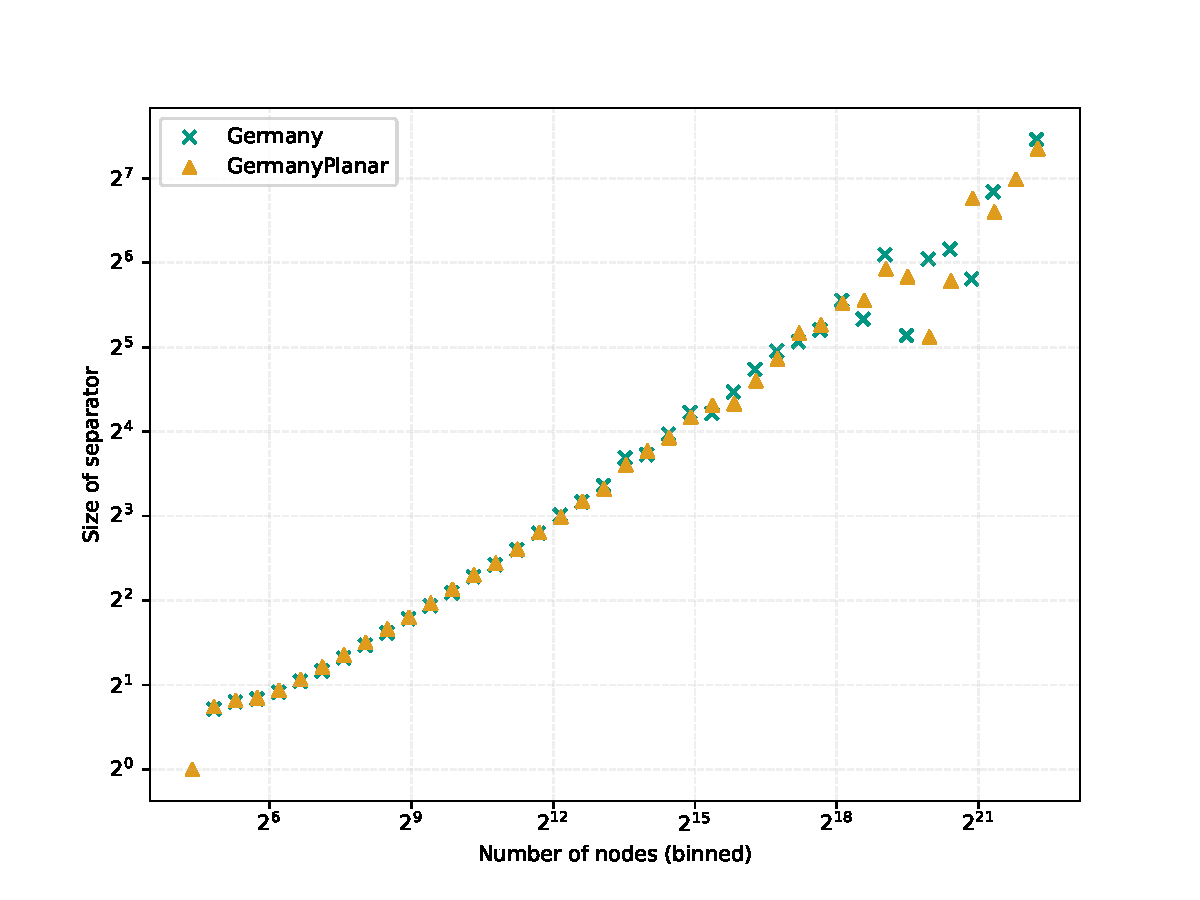
\includegraphics[width=0.8\linewidth]{graphics/GermanyPlanarVsNonPlanar.pdf}
	\caption{Comparison of separator sizes in the German road network: planar vs. non-planar.}
	\label{fig:germany_planar_vs_non_planar}
\end{figure}

Our findings indicate that separators in non-planar road networks closely
resemble those in their planarized versions. Frequently, non-planar separators
are also separators in the planarized graph or can be adapted to planar ones
with the addition of only a few nodes. This can be seen in
\cref{fig:karlsruhe_planar_vs_non_planar}, which depicts a non-planar separator
extended to be a separator in the planarized Karlsruhe network.
\todo{explain they can get larger and smaller}
\todo{also say that separators can increase: simple example two disjoint components that get connected}

\begin{figure}
	\centering
	\begin{subfigure}{0.45\linewidth}
		\centering
		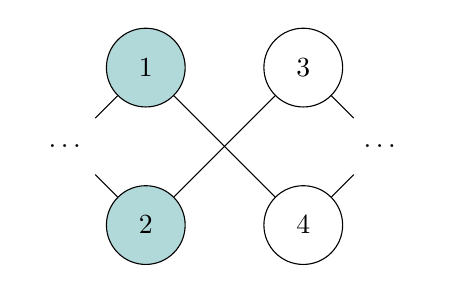
\begin{tikzpicture}[every node/.style={circle, draw, minimum size=1cm}]
			\node[draw=none] (dots1) at (0, 1) {\dots};
			\node[fill=teal!30] (1) at (1, 2) {1};
			\node[fill=teal!30] (2) at (1, 0) {2};
			\node (3) at (3, 2) {3};
			\node (4) at (3, 0) {4};
			\node[draw=none] (dots2) at (4, 1) {\dots};

			\draw (1) -- (4);
			\draw (2) -- (3);

			\draw (1) -- (dots1);
			\draw (2) -- (dots1);
			\draw (3) -- (dots2);
			\draw (4) -- (dots2);
		\end{tikzpicture}
		\caption{Separator in non-planar graph}
	\end{subfigure}
	\hfill
	\begin{subfigure}{0.45\linewidth}
		\centering
		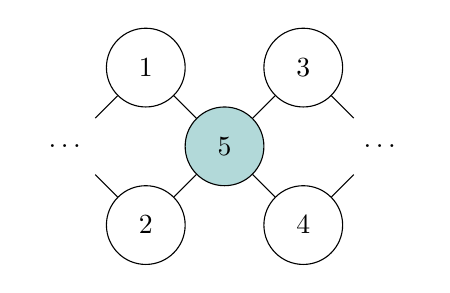
\begin{tikzpicture}[every node/.style={circle, draw, minimum size=1cm}]
			\node[draw=none] (dots1) at (0, 1) {\dots};
			\node (1) at (1, 2) {1};
			\node (2) at (1, 0) {2};
			\node (3) at (3, 2) {3};
			\node (4) at (3, 0) {4};
			\node[fill=teal!30] (5) at (2, 1) {5};
			\node[draw=none] (dots2) at (4, 1) {\dots};

			\draw (1) -- (5);
			\draw (2) -- (5);
			\draw (3) -- (5);
			\draw (4) -- (5);

			\draw (1) -- (dots1);
			\draw (2) -- (dots1);
			\draw (3) -- (dots2);
			\draw (4) -- (dots2);
		\end{tikzpicture}
		\caption{Better separator in planarized graph}
	\end{subfigure}
	\caption{Example of a separator, where a better separator can be found in the planarized graph.}
	\label{fig:planarization_reduces_separator}
\end{figure}

\begin{figure}
	\centering
	\begin{subfigure}{0.45\linewidth}
		\centering
		\begin{tikzpicture}[every node/.style={circle, draw, minimum size=1cm, node distance=1.5cm}]
			\node[fill=teal!30] (1) {1};
			\node[below right=of 1, fill=teal!30] (3) {3};
			\node[left=3cm of 3] (2) {2};
			\node[below left=of 3] (4) {4};

			\draw (1) -- (4);
			\draw (1) -- (2) -- (3);

			\node[right=of 1, draw=none] (dots1) {\dots};
			\node[right=of 4, draw=none] (dots4) {\dots};
			\draw (1) -- (dots1);
			\draw (4) -- (dots4);
			\draw (3) -- (dots4);
			\draw (3) -- (dots1);

			\draw[dashed] (-1, 1) -- (-1, -4.5);
		\end{tikzpicture}
		\caption{Separator in non-planar graph\newline}
	\end{subfigure}
	\hfill
	\begin{subfigure}{0.45\linewidth}
		\centering
		\begin{tikzpicture}[every node/.style={circle, draw, minimum size=1cm, node distance=1.5cm}]
			\node[fill=teal!30] (1) {1};
			\node[below right=of 1, fill=teal!30] (3) {3};
			\node[left=3cm of 3, fill=teal!5] (2) {2};
			\node[below left=of 3, fill=teal!5] (4) {4};
			\node[below= 0.75 of 1, fill=teal!5] (5) {5};

			\draw (1) -- (5);
			\draw (4) -- (5);
			\draw (5) -- (3);
			\draw (1) -- (2) -- (5);

			\node[right=of 1, draw=none] (dots1) {\dots};
			\node[right=of 4, draw=none] (dots4) {\dots};
			\draw (1) -- (dots1);
			\draw (4) -- (dots4);
			\draw (3) -- (dots4);
			\draw (3) -- (dots1);

			\draw[dashed] (-1, 1) -- (-1, -4.5);
		\end{tikzpicture}
		\caption{The separator of the original graph is not a separator in the planarized graph.}
	\end{subfigure}
	\caption{Example where the separator of the original graph is not a separator in the planarized graph.}
\end{figure}



\begin{figure}
	\centering
	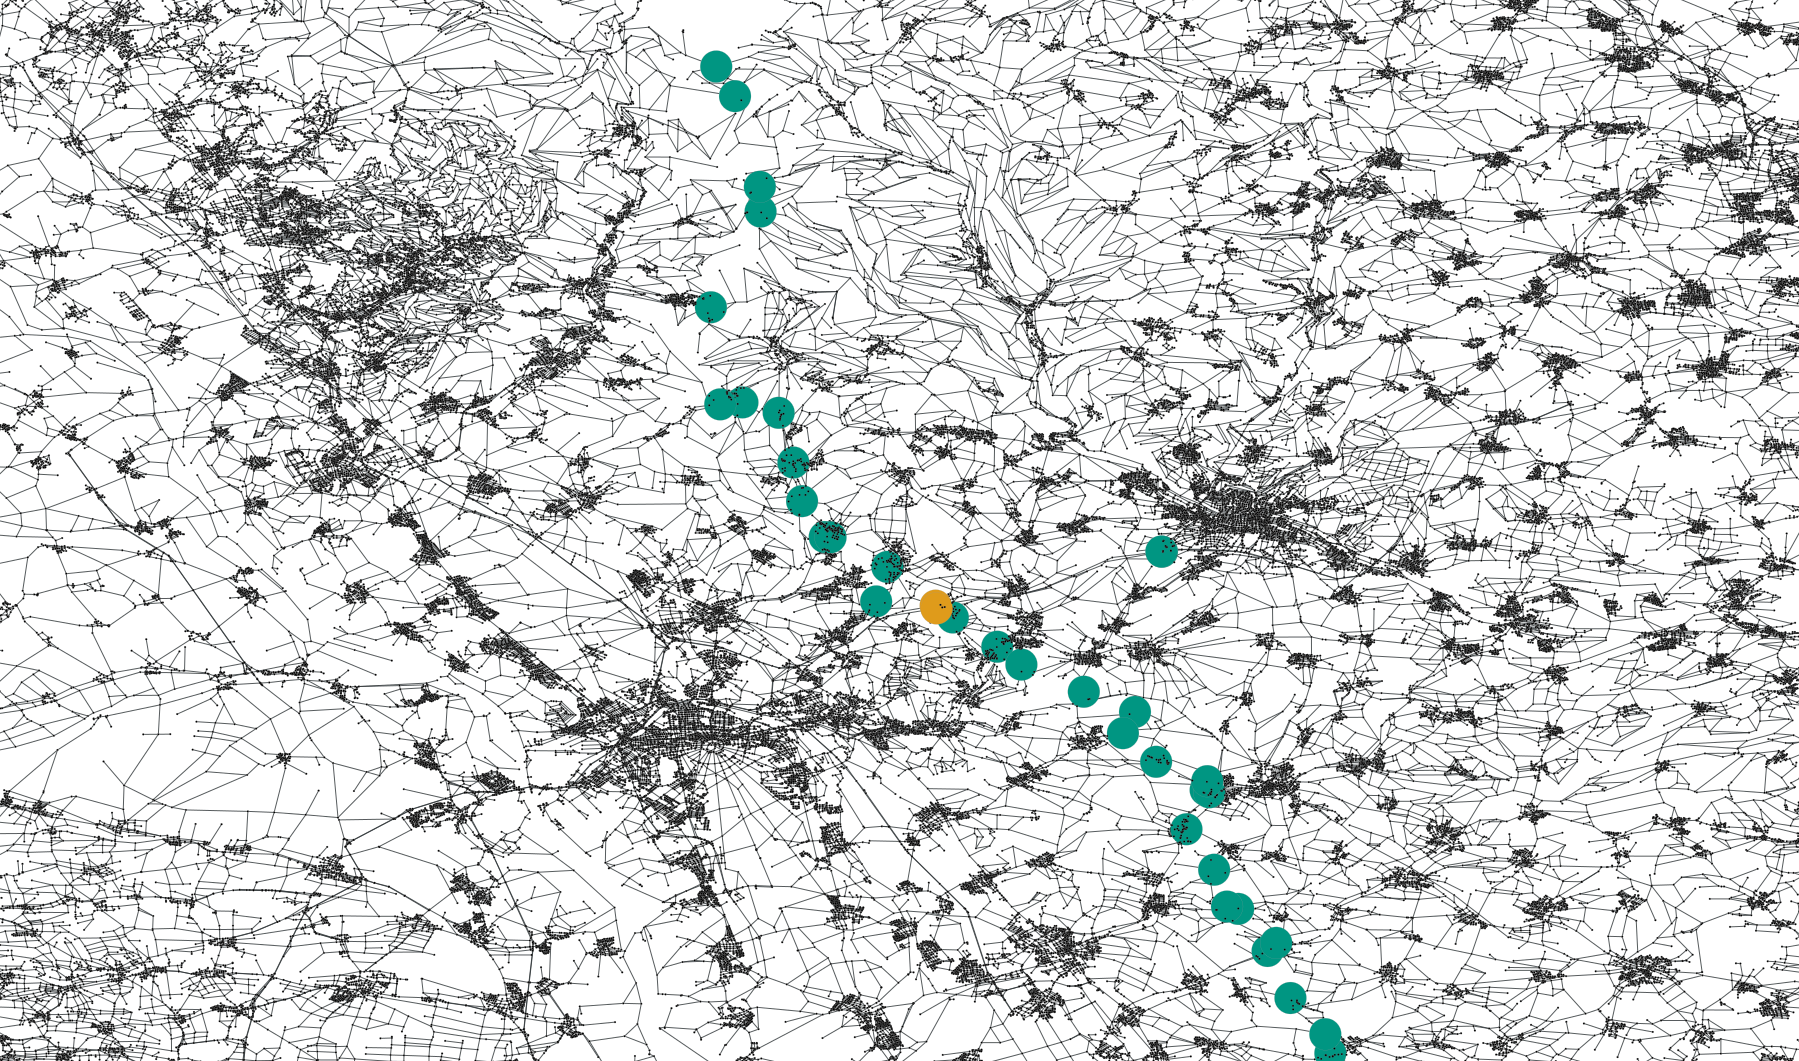
\includegraphics[width=0.8\linewidth]{graphics/karlsruhe_top_level_sep_extended_to_planar_wide.png}
	\caption{Example visualization of one possible top-level separator for
		Karlsruhe. Teal points represent the separator of the original graph, while
		orange points denote the additional nodes required to make it separator
		for the planarized version of Karlsruhe. Separators where computed with
		KaHIP.} \label{fig:karlsruhe_planar_vs_non_planar}
\end{figure}

These findings highlight that the near-planar structure of road networks has
minimal impact on separator size, suggesting that such networks can typically
be analyzed as planar graphs.
